\documentclass{article}
\usepackage{amsfonts, amsmath, amssymb, amsthm} % Math notations imported
\usepackage{enumitem}
\usepackage[margin=1in]{geometry}
\usepackage{graphicx}
\usepackage{subfig}
\graphicspath{{./images/}} % Path to images

\newtheorem{thm}{Theorem}
\newtheorem{prop}[thm]{Proposition}
\newtheorem{cor}[thm]{Corollary}

% title information
\title{Math 154 HW3}
\author{Neo Lee}
\date{04/26/2023}

% main content
\begin{document} 

% placing title information; comment out if using fancyhdr
\maketitle 

\textbf{Problem 1.}
\begin{prop}
    Any tree with $n\ge 2$ vertices has at least 2 leaves.
\end{prop}
\begin{proof}
    Let $P = (v_1, \dots, v_k)$ be the longest path in any arbitrary tree $T$ with $n\ge 2$ vertices.  
    Then, we know that all the neighbors of $v_1$ and $v_k$ must be in $P$.
    Assume for the sake of contradiction that $v_1$ has more than one neighbor, let $v_2, v_r$ be two of them, then $v_2, v_r \in P$, and there would be a cycle $(v_1, v_2, \dots, v_r, v_1)$, which contradicts the definition of tree.
    Hence, $v_1$ has only one neighbor. Similarly, $v_k$ has only one neighbor.
    Therefore, $v_1$ and $v_k$ are the leaves of $T$.
\end{proof}
\bigbreak

\textbf{Problem 2.}
\begin{prop}
    If $G$ is a graph in which there is a unique path between each pair of vertices, then $G$ is a tree.
\end{prop}
\begin{proof}
    We seek to prove that $G$ is connected and acyclic.
    
    Firstly, $G$ is connected because there is a path between each pair of vertices.

    Then, assume for the sake of contradiction that $G$ has a cycle $C = (v_1, \dots, v_k, \dots, v_1)$.
    Then, there are two paths between $v_1$ and $v_k$ with the one path being the first half of $C$ and the other path being the other half of $C$, which contradicts the assumption that there is a unique path between each pair of vertices.

    Therefore, $G$ is a tree.
\end{proof}
\bigbreak

\textbf{Problem 3.}
\begin{enumerate}[label=(\alph*)]
    \item \begin{prop}
        Any forest with $n$ vertices and $k$ components has exactly $n-k$ edges. 
    \end{prop}
    \begin{proof}
        Let $T_1, \dots, T_k$ be the components of the forest. 
        Then, each $T_i$ is a tree, and has $n_i$ vertices and $n_i - 1$ edges.

        Therefore, the forest has $\sum_{i=1}^{k}n_i = n$ vertices and $\sum_{i=1}^{k}n_i-1 = \left(\sum_{i=1}^{k}n_i\right)-k = n-k$ edges.
    \end{proof}

    \item \begin{prop}
        Any n-vertex graph with at least n edges contains a cycle.
    \end{prop}
    \begin{proof}
        Let an arbitrary graph $G$ with $n$ vertices. 
        
        \begin{enumerate}[label=Case \arabic*:]
            \item 
            If $G$ is connected. Assume for the sake of contradiction that $G$ has no cycle. 
            Then, $G$ is a tree, and has $n-1$ edges, which contradicts the assumption that $G$ has at least $n$ edges.
            Hence, $G$ must have a cycle.

            \item 
            If $G$ is not connected. Let $G_1, \dots, G_k$ be the components of $G$.
            
            Now assume for the sake of contradiction that all components $G_i$ have $|E(G_i)| < |V(G_i)|$.
            However, notice that all components are disjoint, so $\sum_{i=1}^{k}|E(G_i)| \ge \sum_{i=1}^{k}|V_(G_i)|$, which is impossible under our contrary assumption.
            Hence, there must exist $G_j$ such that $|E(G_j)| \ge |V(G_j)|$.
            Then, consider only that component $G_j$, and with the same argument from Case 1, there is a cycle in $G_j$.
        \end{enumerate}
    \end{proof}
\end{enumerate}
\pagebreak

\textbf{Problem 4.}
\begin{enumerate}[label=(\alph*)]
    \item 
    \indent
    \begin{figure}[h!]
        \qquad
        \begin{minipage}{.4\textwidth}
            \centering
            {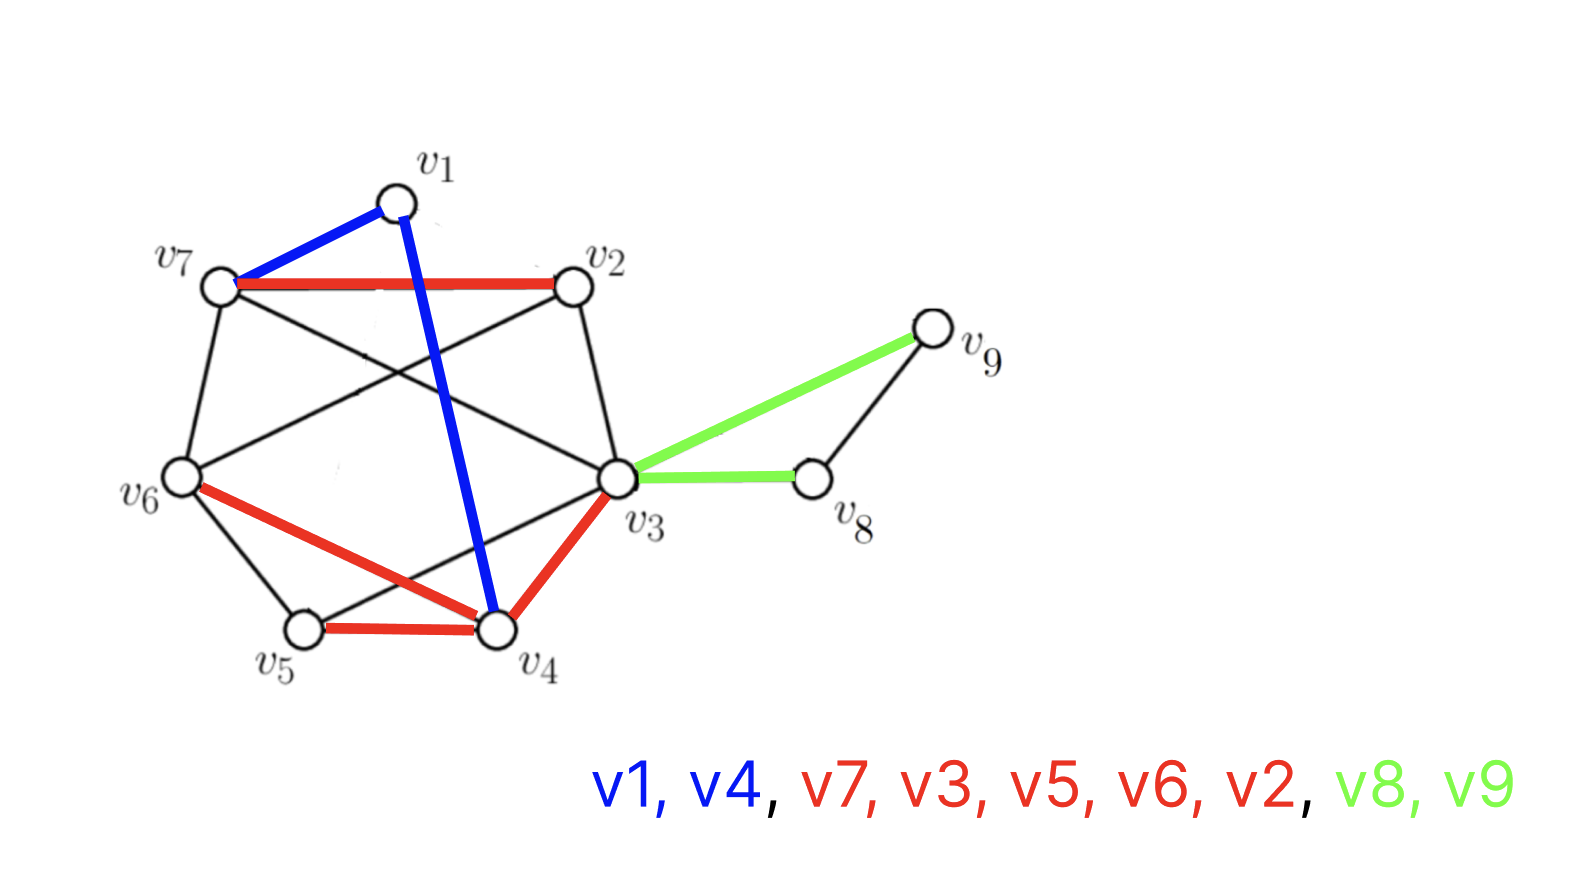
\includegraphics[scale=0.25]{BFS.png}}
            \qquad\qquad\emph{BFS}\label{fig:1}
        \end{minipage}    
        \qquad
        \begin{minipage}{.4\textwidth}
            \centering
            {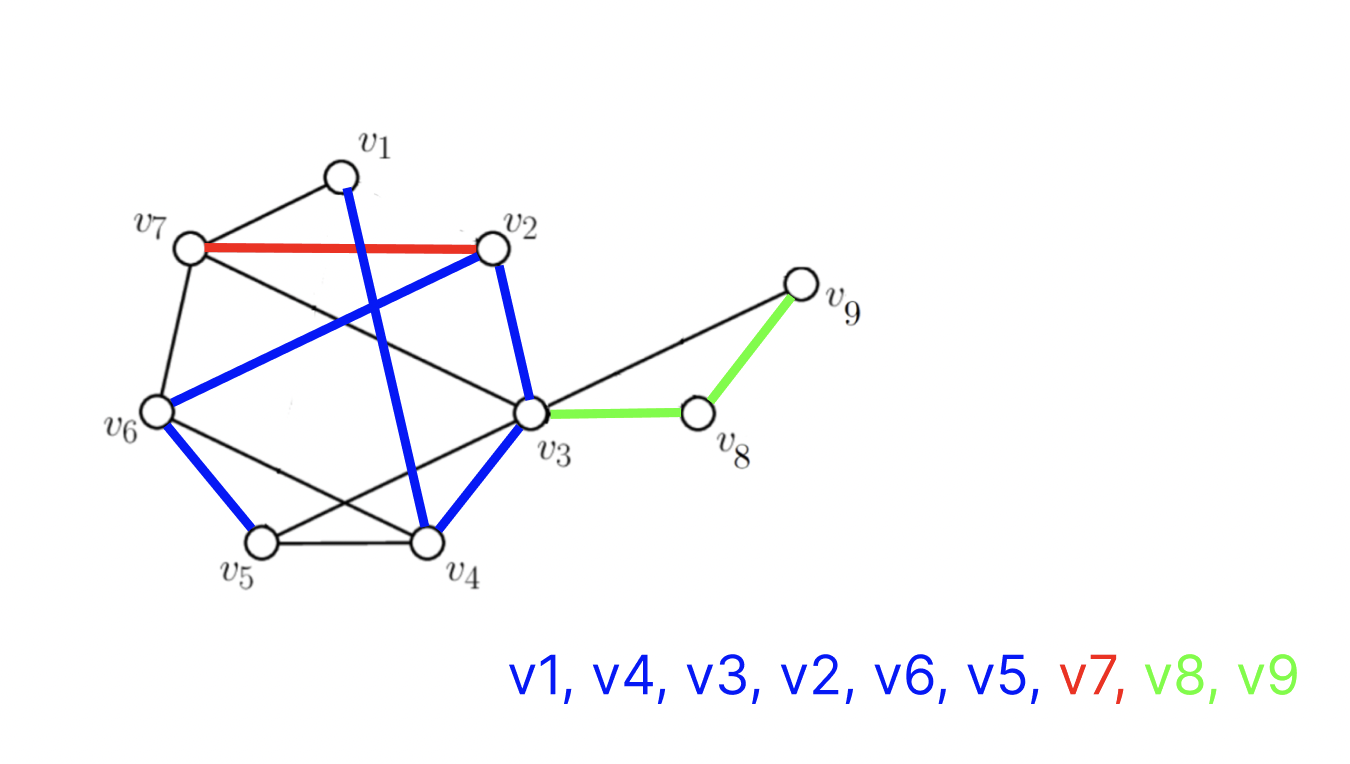
\includegraphics[scale=0.3]{DFS.png}}
            \qquad\qquad\emph{DFS}\label{fig:2}
        \end{minipage}        
    \end{figure} 

    \item
    Height of the BFS tree is 3, and height of the DFS tree is 5.

    \item
    Radius of the graph is 2.

    \item
    Diameter of the graph is 3.
\end{enumerate}
    


\end{document}